\documentclass[12pt,english]{article}
\usepackage[latin9]{inputenc}
\usepackage{geometry}
%\usepsackage{babel}
\usepackage{amsthm}
\usepackage{amsmath}
\usepackage{amssymb}
\usepackage{graphicx}
\usepackage{setspace}
\usepackage{hyperref}
 \usepackage{cleveref}
 \usepackage{topcapt, lscape}
 \usepackage{rotating}
 \usepackage{booktabs}
 \usepackage[para]{threeparttable}
%\usepackage{breakurl}
\usepackage{color}
\usepackage{harvard}
\usepackage{float}
\usepackage{topcapt, lscape}
%\setcounter{MaxMatrixCols}{10}
\usepackage{scalefnt}
%\usepackage{ulem}
\newcommand{\note}[1]{\footnote{ \begin{doublespace}#1  \end{doublespace}}}

\usepackage[para]{threeparttable}
\geometry{verbose,tmargin=1.25in,bmargin=1.25in,lmargin=1in,rmargin=1in}
\setlength{\parskip}{0.1in}
\setlength{\parindent}{0pt}
\makeatletter
\newcommand{\lyxdot}{.}
\numberwithin{equation}{section}


\theoremstyle{plain}
\newtheorem{thm}{\protect\theoremname}

\newtheorem{assumption}{\protect\assumptionname}
\theoremstyle{remark}

\newtheorem*{rem*}{\protect\remarkname}
\newtheorem{rem}{\protect\remarkname}[section]
  \theoremstyle{plain}

\newtheorem{lem}{\protect\lemmaname}
  \providecommand{\assumptionname}{Assumption}
  \providecommand{\lemmaname}{Lemma}
  \providecommand{\remarkname}{Remark}
\providecommand{\theoremname}{Theorem}
\makeatother
  \providecommand{\assumptionname}{Assumption}
  \providecommand{\lemmaname}{Lemma}
  \providecommand{\remarkname}{Remark}
\providecommand{\theoremname}{Theorem}
\newcommand{\red}[1]{\textcolor{red}{#1}}
\newcommand{\blue}[1]{\textcolor{blue}{#1}}


\begin{document}

\subsection{Legislative Candidates  \label{candidates}}


%Differently from closed-list PR systems, 
Brazil's electoral system puts individual candidates at the center of political choice. Indeed, the literature notes that (i) parties are weak, under-resourced, and often unable to constrain opportunistic behavior by individual legislators \cite{Samuels2003,Desposato2006,KlavsnjaTitiunik2017}; (ii) open-list PR and a lack of formal mechanisms channeling resources to congressional party leaders promote candidate-centric legislative careers \cite{Mainwaring1995,Samuels2003}; and (iii) %presidents have systematically used pork and cabinet positions to ``buy''   legislative support, leading to what is known as presidential coalitionism \cite{Neto1998,Neto2006}; and (iv) 
Brazilian elections tend to be candidate-centric rather than party-centric, with voters effectively responding to candidate characteristics above party labels \cite{Mainwaring1995,Samuels2003,KlavsnjaTitiunik2017}.

Understanding the drivers of voters' choices, therefore, requires that we analyze them at the candidate level. %, as opposed to the party-level.
To that end, we bring together data on candidates running for a seat in the C\^{a}mara dos Deputados in the 2006, 2010, and 2014 elections. In total, across these three elections and all 27 legislative districts, there were 15,698 candidate-years: 4,944 in 2006, 4,887 in 2010, and 5,867 in 2014.  For each candidate running for office, we observe the number of votes obtained by the candidate in each municipality, along with a % \red{(from source)}. For the vast majority of these candidates, we observe a 
 rich set of individual characteristics including their previous professional and political experience, level of education, and gender.\note{\normalsize This information is available from the \emph{Tribunal Superior Eleitoral} (TSE).} %\note{\normalsize \red{For details on coding, and additiional descriptive statistics, see Appendix XXX}} %For more than two thirds of all candidates (10752 across the three elections), we are also able to obtain a measure of their policy position using individual contributions, following the methodology outlined in \citeasnoun{Bonica2014}. We describe this in detail below. 
For 10,025 of these candidates, we are also able to estimate a measure of their policy positions using individual campaign contributions.

Figure \ref{fig:selectiononvalence} provides summary statistics of candidates' observable non-policy  characteristics.\note{following standard practice, we refer to these non-policy attributes as valence.} Overall, we find that incumbents constitute only a fraction of all candidates,but are disproportionately represented among candidates who secure a seat in the chamber. While only about half of the candidates have higher education, this figure increases to about 75\% for elected candidates; women compose only about a quarter of total candidates, but an even far lower percentage of elected candidates; candidates with business or government (bureaucratic) experience  make about 10\% of the pool of candidates, and they represent a significantly lower proportion of elected candidates. %Figure \ref{desccorrels} further highlights these differences for incumbency, education, gender, and age in terms of candidates' vote shares.  

\begin{figure}[h]
   \centering
   \includegraphics [height=12cm] {\lyxdot /Presentation/figs/candidate/valence_elected_nonelected.pdf}
   \caption{Candidates Observable Non-Policy (Valence) Characteristics.}
   \label{fig:selectiononvalence}
\end{figure}

%\begin{figure}[h]
%\begin{center}$
%\begin{array}{cc}
 %\includegraphics [width=6.7cm,height=5cm] {\lyxdot /presentation/figs/matifigs/voteshare_byincumbent.jpg} &
%\includegraphics[width=6.7cm,height=5cm]{\lyxdot /presentation/figs/matifigs/voteshare_byhigheredu.jpg} \\
%\text{Incumbency} & \text{Higher Education} \\ 
 %\includegraphics [width=6.7cm,height=5cm] {\lyxdot /presentation/figs/matifigs/voteshare_by_genderfem.jpg} &
%\includegraphics[width=6.7cm,height=5cm]{\lyxdot /presentation/figs/matifigs/voteshare_age_crossplot.jpg} \\
%\text{Gender (female)} & \text{Age} \\
%\end{array}$
%\end{center}
%\caption{Candidate Vote Shares (among registered district voters) by Valence Attribute.}
%\label{desccorrels}
%\end{figure}

Education, professional experience, gender, and other valence attributes of candidates are clearly important to voters. Policy positions candidates adopt matter as well. This has been documented in the U.S.\ and elsewhere.\note{\normalsize See, e.g, \citeasnoun{Canes-Wrone-etal2002}, \citeasnoun{AnsolabehereJones2010}, and \citeasnoun{Iaryczoweretal2018}.} In Brazil, there is growing evidence of the strengthening of programmatic parties and policy position \citeasnoun{Hagopian2009}. These defined policy positions can alter voting behavior, but defining the extent to which voters respond to these changes has been fraught by a set of challenges which we address in this exercise.

Estimating how voters' preferences for candidates vary with the policies endorsed by legislative candidatess requires a measure of both elected and non-elected candidates' policy positions. Unfortunately, there are currently no available measures of both incumbents' and challengers' policy positions for Brazilian legislative elections.\note{\normalsize \citeasnoun{Zucco2009} and \citeasnoun{ZuccoLauderdale2011} estimate \emph{incumbents}' ideal points using surveys that ask them to place themselves and all the main political parties represented in the legislature on a left-right, ten-point scale. As these scholars note, estimation of incumbents' ideal points via DW-Nominate is challenging due to widespread ``vote-buying'' of legislators through pork-barrel spending and cabinet allocations.} %\note{\normalsize \citeasnoun{Zucco2009}, \citeasnoun{ZuccoLauderdale2011}, and \citeasnoun{PowerZucco2012} estimate \emph{incumbents}' ideal points using surveys that ask them to place themselves and all the main political parties represented in the legislature on a left-right 10-point scale (see \citeasnoun{Power2010}). As these papers suggest, estimation of incumbents' ideal points via DW-Nominate is problematic due to widespread ``vote-buying'' of legislators through pork-barrel spending and cabinet allocations.} 
To address this gap, we adopt the estimation approach of \citeasnoun{Bonica2014} and produce novel estimates of candidates' policy choices, using micro-level data on campaign contributions for 2004-2014.\note{\normalsize In U.S.\ data, Bonica's estimates closely match ideal point estimates obtained using row call data.} The key assumption is that a contributor's marginal benefit of giving to a candidate is decreasing in the distance between the contributor's ideal policy and the candidate's choice. Through an augmented correspondence analysis, we use these campaign contributions to estimate individual policy positions across candidates, pooling available data for the entire period.\note{Details of the estimation and robustness checks can be found in Appendix \ref{cfcore_appendix}.} The intuition is that candidates who receive campaign donations from the same contributors -- and similar amounts -- should be close with respect to their policy positions.\note{\normalsize While Bonica interprets these estimates as politicians' preferred policies, we  only make the assumption that these are the candidates' policy choices, which could or not correspond to their true preferences.} Conversely, if patterns of contributions are dissimilar, these differences translate into a greater distance in their policy positions.
    
% The intuition for estimation is as follows. For each candidate $j$, she receives a vector of campaign donation from a subset of voters. Intuitively, if two political candidates receive donations from the same ssubset of voters, in the same amount, we presume them to be close to each other deologically. Correspondance analysis allowss us to rduce thees multidimensional patterns of campaign contributionss into a one-dimensional Estimation is carried out with an augmented correspondence analysis with a two-way frequency matrix, where rows correspond to unique contributors and columns to candidates.\note{Correspondance analysis is a statistical method that decompoess multidimensional contingency matrices into a set of eigenvectors, usualy } Each element in the matrix is the total amount of contributions made by contributor $i$ to candidate $j$, for the time span of our data. We then perform a singular value decomposition to retrieve ideal points for contributors and recipients.
    
    
%The intuition for how campaign contributions can be used to estimate politicians' policy positions is similar in spirit to that behind DW-Nominate. % In the latter, $K$ legislators face a sequence of decisions between two alternatives, which are unobservable for the econometrician. If legislators' ideal points were known, we can think of the estimation problem as finding separating hyperplanes (or midpoints in one dimension) that minimize incorrect classification of predicted yay and nay votes. If instead all separating hyperplanes were known, ideal points for each legislator are again found by minimizing classification errors across roll calls. We can think of an algorithm behind DW-Nominate as alternating between one and the other step, until convergence. With campaign contribution data, each contributor takes the role of a roll call, and their contributions of the separating hyperplanes (extended, of course, from a binary choice to a continuum). 
% The key assumption is that the contributor's marginal benefit of giving to a particular candidate is decreasing in the distance between the contributor's ideal policy and the candidate's choice. This implies that contributors give (weakly) more money to candidates that are closer to their ideal point, which in turn allows us to rank candidates' positions in the policy space. Bonica interprets these estimates as politicians' policy preferences. We only make the assumption that these are the candidates' policy choices, which could or not correspond to their true preferences. %\note{\normalsize Estimation is carried out by a modified correspondence analysis with a two-way frequency matrix, where rows correspond to unique contributors and columns to candidates. Each element in the matrix is the total amount of contributions made by contributor $i$ to candidate $j$, for the time span of our data. We then perform a singular value decomposition to retrieve ideal points for contributors and recipients.}  

We rely on rich micro-level data on dyadic contributions, which include both individual and corporate donations and to which politician they have donated.\note{\normalsize The campaign contribution data is available since the 2000 election, when the TSE mandated the disclosure of electoral campaign contributions to candidates at all levels of government.% Importantly, the dataset uniquely identifies both contributors and recipients.
}  Since corporations may donate to candidates strategically to secure access, we exclude them from our data and focus on individual contributions by non-partisans and non-politicians. In total, we leverage data from over 650 thousand unique contributions at the federal level, and 3.8 million unique contributions at the local level, pooling across electoral cycles.%\note{\normalsize We estimate scores separately for local and federal candidates, pooling across electoral cycles.} %\note{\normalsize Federal and state-level elections occur in Brazil every four years, at a two-year interval from municipal elections.}  
\note{\normalsize Under-the-table donations---\emph{caixa dois}---are common, but previous research using the same data shows that officially declared donations capture the majority of campaign contributions \cite{BoasHidalgoRichardson2014}.} Because many non-viable candidates tend to receive no individual-level contributions, we are forced to drop a sizable number of candidates from the database. Nevertheless, our final sample includes % we are able to provide policy position estimates for more than two thirds of all candidates running for office, totaling
10,025 candidates across the three elections.\note{\normalsize The candidates for whom we are able to recover policy positions make an overwhelming fraction of all candidates seriously contending for a seat in the  C\^{a}mara dos Deputados---see Figure \ref{fig:smallpeople} in the Appendix. In fact, only 0.2\% of candidates for whom we don't have policy data were ultimately elected. Table \ref{coverage} in the Appendix summarizes coverage of the final dataset by state and electoral cycle.}

Figure \ref{cfscore_hist} presents the candidate-level policy positions estimated from campaign donations as well as the spreads across parties across all electoral cycles. We note that candidates tend to center their policy positions around the median, with relatively flat tails in the distribution. Moreover, candidates seem to be on the whole balanced acros both sides of the political spectrum, although with a relatively larger mass to the right. Additionally, traditionally leftist parties such as PT and PSOL attract candidates whose policy positions gravitate to the left, while right parties such as DEM and PDSB have candidates who lean farther to the right.

% \begin{figure}[H]
%   \begin{center}
%     \includegraphics[height=8cm,width=12cm]{\lyxdot ./figs/histogram_pooled_cfscore.pdf}
%   \caption{Distribution of policy positions across politicians. Sample includes federal, state and local-level candidates (2000-2014).}
%   \label{fig:cfscore_hist}
% \end{figure}


\begin{figure}[h]
  \centering
  \includegraphics[height=6cm,width=6cm]{\lyxdot /Presentation/figs/ideology/histogram_pooled_cfscore.pdf}
  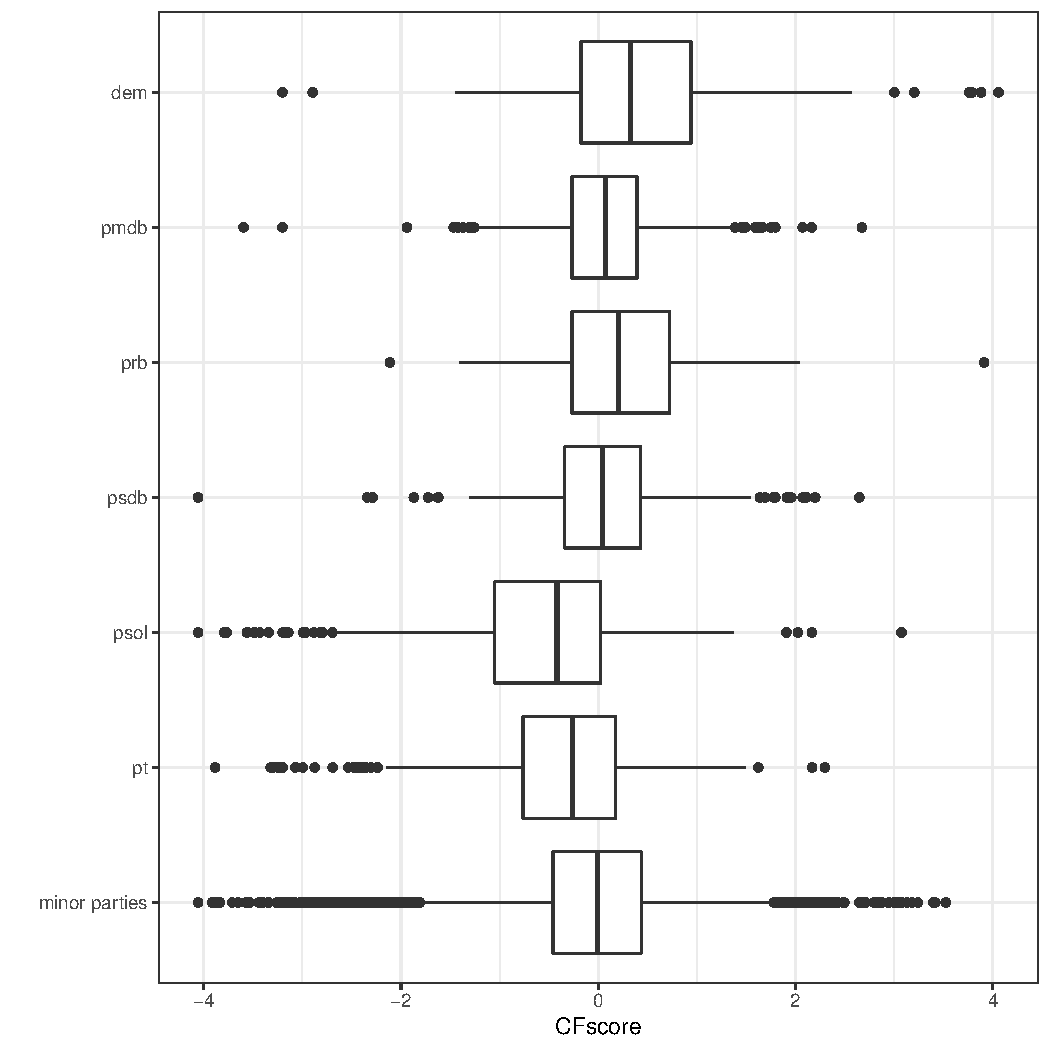
\includegraphics[height=6cm,width=6cm]{\lyxdot /Presentation/figs/ideology/cfscore_pooled_by_party.pdf}
  \caption{Distribution of policy positions. Histogram of all individual-level policy possitions (left) and by party (right), highlighting major parties such as PT, PMDB and DEM.}
  \label{fig:cfscore_hist}
\end{figure} 

We perform a battery of sanity checks of the external and internal validity of our candidate policy estimates.  The left panel of figure \ref{fig:sanitycheck1} in the Appendix shows that there is a strong correlation between policy positions within the same party at both the local and federal level. The right panel of the same figure shows that our policy estimates are correlated with the ideology scores estimated by \citeasnoun{Zucco2009}  at the party level. Figure \ref{fig:sanitycheck2}, on the other hand, shows that our estimates capture the leftward ideological shift of voters and parties in the 2000s found in Latinobarometer surveys. Figure \ref{fig:cfscore_percentile} shows that our stimates are robust to excluding top 5 and 10 percentile donors. Lastly, figure \ref{fig:campaign_contract} shows that individual level contracts do not correlate with total earmarks by federal deputy.%, % \cite{ZuccoLauderdale2011}.  % This is consistent with the findings of \citeasnoun{Bonica2014} for the U.S.

In the next section, we use this information on candidates' valence characteristics and policy choices, along with election results, to estimate voters' preferences. Voters can in principle give their vote to any candidate in the district but choose someone with particular attributes. Another alternative that is de facto available to voters is to abstain or to cast a void vote. This ``outside option'' is thus effectively competing with all the candidates for votes. As Figure  \ref{fig:abstention} illustrates, this, in itself, is a formidable alternative. The 29\% average abstention rate and 8.6\% average blank vote rate in what is formally a compulsory voting system provide suggestive evidence that voters are not enthusiastic about the candidates they face.

\begin{figure}[h]
   \centering
   \includegraphics [width=12cm] {\lyxdot /Presentation/figs/matifigs/abstention_and_blank_h.jpg}
   \caption{Distribution of Abstention and Blank Vote Shares (among registered voters) in Each Municipality, by State (2014).}
   \label{fig:abstention}
\end{figure}

\newpage

{\linespread{1} \small  \bibliographystyle{econometrica}
\bibliography{\lyxdot choicesetbib}}
\end{document}